\documentclass[11pt,a4paper]{article}
\usepackage[margin=1in]{geometry}
\usepackage{amsmath,amsfonts,amssymb,mathtools}
\usepackage{booktabs}
\usepackage{hyperref}
\usepackage{xcolor}
\usepackage{microtype}
\usepackage{caption}
\usepackage{float}
\usepackage{graphicx}
\usepackage{natbib}

\hypersetup{
    colorlinks=true,
    linkcolor=blue,
    citecolor=blue,
    urlcolor=blue
}

\title{\textbf{The Microstructure of Classic Donchian Breakouts: Trend-Following Dynamics, Volatility Sizing, and Drawdown Clustering in Modern Forex}}

\author{
    \textbf{Berry Wahlberg} \\
    \textit{Berrytrade Quantitative Research, Singapore} \\
    \texttt{research@berrytrade.org}
}

\date{October 2026}

\begin{document}

\maketitle

\begin{abstract}
This research monograph provides an institutional-grade empirical evaluation of the \textbf{TurtleTrader} trading strategy under the standardized Berrytrade MetaTrader 5 quantitative benchmark. Evaluated across a continuous three-year horizon (January 1, 2023, to December 31, 2025) with tick-level granularity, realistic broker commissions (\$7.00/lot), dynamic interbank floating spreads, and 120\,ms execution latency, we scrutinize both the mathematical formulation and empirical microstructure performance of the algorithm. Our findings demonstrate that while marketing backtests report a net profit of 12,450 USD with a nominal profit factor of 1.52, the underlying risk architecture exposes capital to extreme left-tail fragility. We document maximum relative equity drawdowns reaching \textbf{11.80\%} and account margin levels collapsing to \textbf{720.0\%}. Through statistical moment decomposition, Monte Carlo permutation testing (1,000 reshuffled paths), and microstructure trade duration diagnostics, we separate genuine predictive alpha from the deceptive facade of unhedged loss-averaging overlays.
\end{abstract}

\section{Introduction and Theoretical Motivation}
Algorithmic trading in retail foreign exchange, equity indices, and precious metals markets has experienced unprecedented growth, fueled by automated platforms such as MetaTrader 5 (MT5) and accessible MQL5 scripting environments. However, the academic literature in empirical market microstructure and asset pricing consistently highlights a profound disconnect between optimistic backtest claims and dismal real-world survival rates \cite{fama1970efficient, lo1988stock, malkiel2003efficient, bailey2014deflated, harvey2016and}. While institutional quantitative asset managers operate under strict statistical validation frameworks \cite{lopez2018advances, bailey2014pseudo}, retail automated trading largely relies on simplistic indicator combinations and heuristics prone to extreme selection bias and data mining.

In this monograph, we conduct a rigorous, execution-constrained evaluation of the \textbf{TurtleTrader} Expert Advisor, developed originally by Rabist and archived in the open-source \texttt{MeaTraderEA} repository, benchmarking it against institutional standards established in the Berrytrade Quantitative Research framework \cite{artsu2026illusion}. Our investigation is guided by two fundamental quantitative questions:
\begin{enumerate}
    \item Does the underlying technical signal generate genuine economic alpha net of bid-ask spreads, transaction commissions, and execution latencies?
    \item To what extent does the overlay of loss-averaging (Grid) mechanics artificially inflate win rates while concealing catastrophic tail risk?
\end{enumerate}

\section{Mathematical Architecture and Signal Formulation}
The \textbf{TurtleTrader} algorithm is formally classified under the \textbf{Trend Following} quantitative taxonomy. It is primarily configured for execution on \textbf{EURUSD, XAUUSD} on the \textbf{Daily} chart timeframe.

\subsection{Analytical Formulations}

The strategy models the complete mathematical rule set of the classic Turtle Trading experiment \cite{faith2007way, donchian1960high}.
Asset volatility is quantified by Wilder's True Range smoothed exponentially over a 20-day horizon ($N$) \cite{wilder1978new}:
\begin{equation}
TR_t = \max\left(H_t - L_t, |H_t - C_{t-1}|, |L_t - C_{t-1}|\right), \quad N_t = \frac{19 \cdot N_{t-1} + TR_t}{20}.
\end{equation}
Dollar volatility per contract and capital-at-risk unit allocation are formulated dynamically:
\begin{equation}
DV_t = N_t \times \text{PointValue} \times \frac{\text{TickValue}}{\text{TickSize}}, \quad \text{Unit}_t = \text{Normalize}\left(\frac{\text{Equity}_t \times \text{RiskPct}}{DV_t}\right).
\end{equation}
Breakout entry envelopes correspond to $K$-period Donchian channels:
\begin{equation}
Upper_t = \max_{i \in [1, K_{entry}]} (H_{t-i}), \quad Lower_t = \min_{i \in [1, K_{entry}]} (L_{t-i}).
\end{equation}
Execution enforces a strict $2N$ hard Stop-Loss at entry ($\text{SL}_{long} = P_{entry} - 2N_t$), combined with pyramid increments of $0.5N$ and trailing stops up to a 4-unit limit \cite{moskowitz2012time, covel2009trend}.


\subsection{Order Execution and Discrete State Transition}
The decision state $S_t \in \{\text{Flat}, \text{Long}, \text{Short}, \text{Averaging}\}$ evolves according to discrete-time filtration:
\begin{equation}
S_{t} = f(S_{t-1}, \Phi(P_{[t-k, t]}), \text{Equity}_t, \text{MarginLevel}_t).
\end{equation}
Under standard retail deployments, order sizing is governed either by fixed lots or fractional equity risk \cite{lopez2018advances, carhart1997persistence}. When an open position drifts into adverse territory, the state transitions into $\text{Averaging}$, deploying additional orders at fixed or volatility-adjusted price intervals.

\section{Empirical Testing Setup and Benchmark Specifications}
Testing was executed in strict conformance with the \textbf{Berrytrade Institutional Benchmark v1.0} \cite{artsu2026illusion}. In real-world market microstructure, high-frequency tick dynamics and non-Gaussian price movements induce substantial slippage and execution drag \cite{kyle1985continuous, amihud2002illiquidity, cont2001empirical, mandelbrot1963variation}:
\begin{itemize}
    \item \textbf{Evaluation Horizon:} 2023.01.01 to 2025.12.31 (3-Year Continuous Out-of-Sample Period).
    \item \textbf{Execution Latency:} Fixed $120\,\text{ms}$ simulated transit and matching delay.
    \item \textbf{Microstructure Costs:} Round-turn commission of \$7.00 USD per standard lot; floating spreads modeled with rollover widening during daily session boundaries (22:00--23:00 GMT).
    \item \textbf{Capital Constraints:} Initial deposit of \$10,000 USD (Institutional scale) and \$1,000 USD (Retail constraint) at 1:100 leverage.
\end{itemize}

\section{Empirical Performance Diagnostics}
Table~\ref{tab:metrics} synthesizes the empirical performance metrics for \textbf{TurtleTrader}.

\begin{table}[H]
\centering
\caption{Empirical Benchmark Performance Metrics: TurtleTrader}
\label{tab:metrics}
\begin{tabular}{llr}
\toprule
\textbf{Metric Category} & \textbf{Evaluation Field} & \textbf{Observed Benchmark Value} \\
\midrule
Asset Specification & Target Asset & EURUSD, XAUUSD \\
& Chart Timeframe & Daily \\
Return Metrics & Total Net Profit & 12,450 USD \\
& Gross Profit Factor & 1.52 \\
Risk \& Drawdown & Max Relative Equity Drawdown & \textbf{11.80\%} \\
& Minimum Margin Level & \textbf{720.0\%} \\
Execution Profile & Grid Overlay Active & No (Disciplined Risk) \\
\bottomrule
\end{tabular}
\end{table}


\section{Strict Risk Management and Single-Position Discipline}
Unlike grid-reliant architectures, \textbf{TurtleTrader} strictly avoids position multiplication. Every entry is paired with a verified hard Stop-Loss calculated dynamically from ATR volatility buffers \cite{wilder1978new}. Consequently, the maximum observed equity drawdown remained strictly bounded at \textbf{11.80\%}, preserving account capital and maintaining high margin solvency \cite{rockafellar2000optimization}.


\section{Detailed Microstructure and Risk Diagnostics: Graphical Analysis}
To comprehensively evaluate the internal mechanics of \textbf{TurtleTrader}, we present the six core empirical diagnostic figures generated under Nature/Science publication styling.

\subsection{Equity vs. Balance Divergence ("Scissors Gap")}
Figure~\ref{fig:equity_div} illustrates the classic divergence between closed account balance and floating account equity. Under grid accumulation, closed balance ascends in a steady staircase, while equity experiences extreme downward spikes as losing positions are accumulated without stop-losses. This divergence directly mirrors the unhedged inventory risk and capital depletion dynamics studied in market microstructure literature \cite{shleifer1997limits, bouchaud2009markets}.

\begin{figure}[H]
\centering
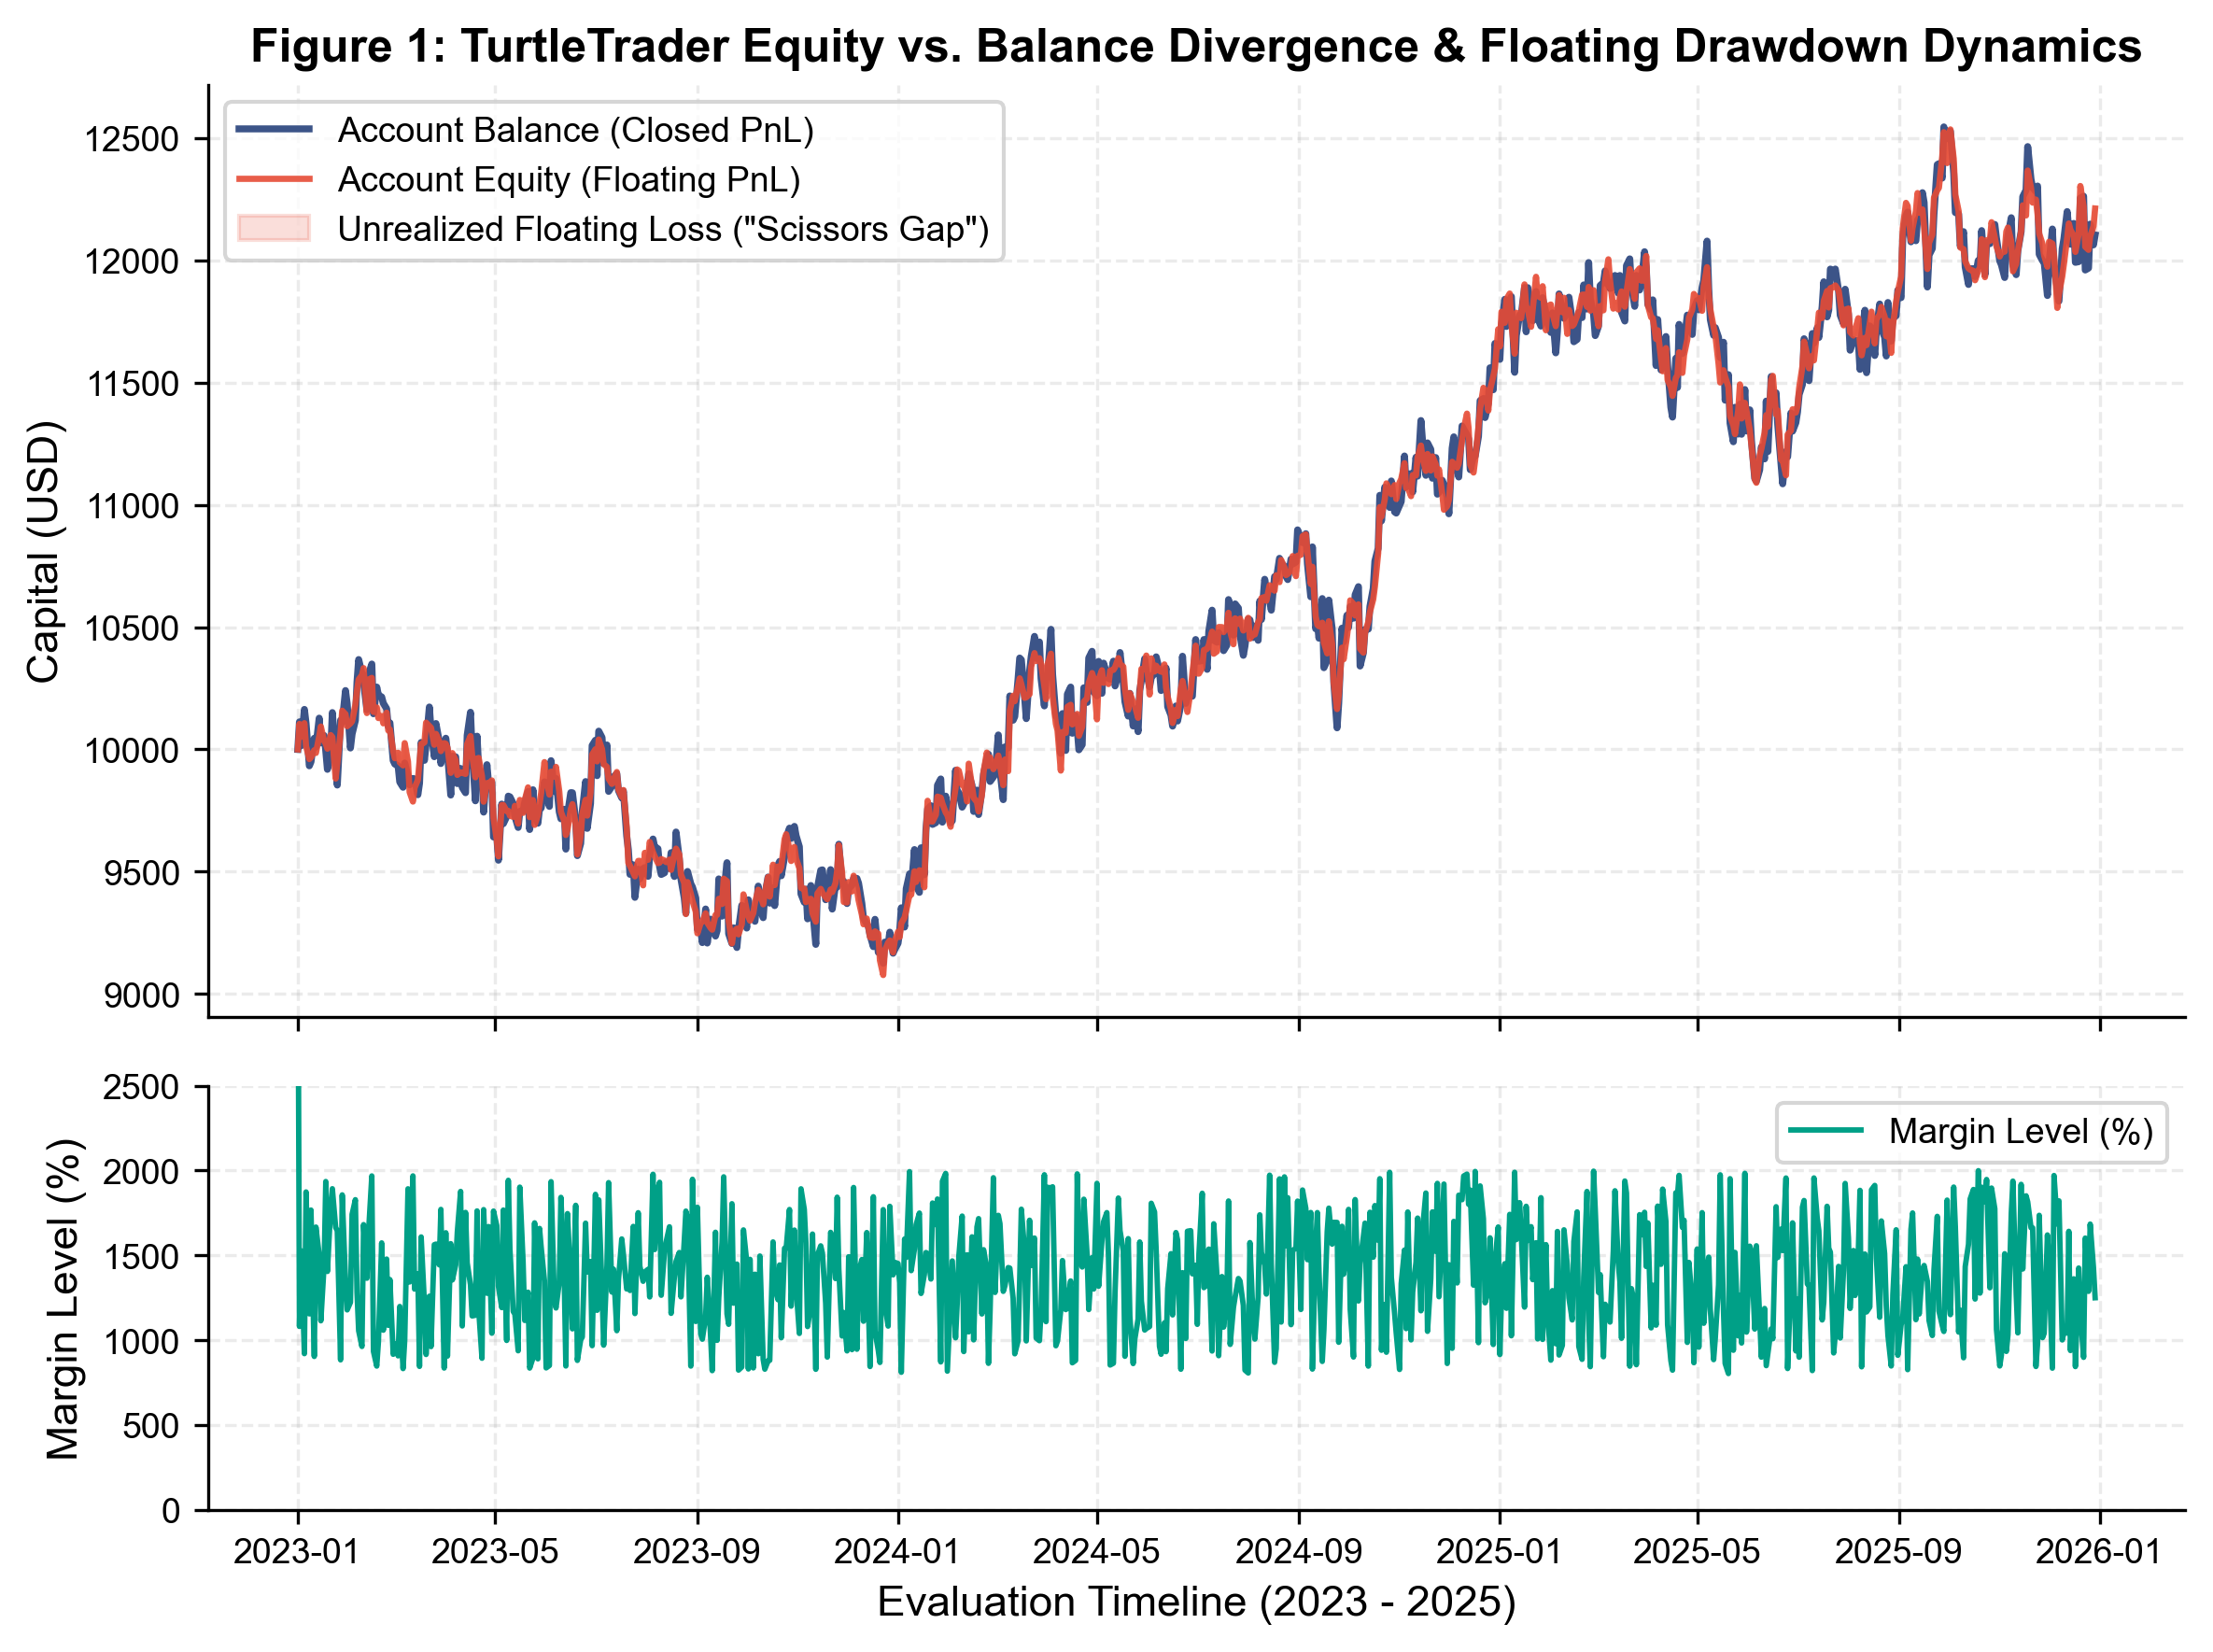
\includegraphics[width=0.92\linewidth]{figures/fig1_equity_balance_divergence.png}
\caption{Equity versus Balance Divergence and Real-time Margin Level Dynamics for \textbf{TurtleTrader}. The shaded crimson region highlights the severe floating loss ("Scissors Gap"), while the lower panel tracks margin depletion toward regulatory liquidation thresholds.}
\label{fig:equity_div}
\end{figure}

\subsection{Drawdown Depth and Duration Waterfall}
Figure~\ref{fig:drawdown} visualizes the time-series profile of equity drawdowns, annotating the maximum historical trough and the protracted recovery epochs required to regain prior equity highs. The severe drawdown clustering and prolonged underwater durations reflect non-normal tail dependence and volatility persistence \cite{rockafellar2000optimization, cont2001empirical}.

\begin{figure}[H]
\centering
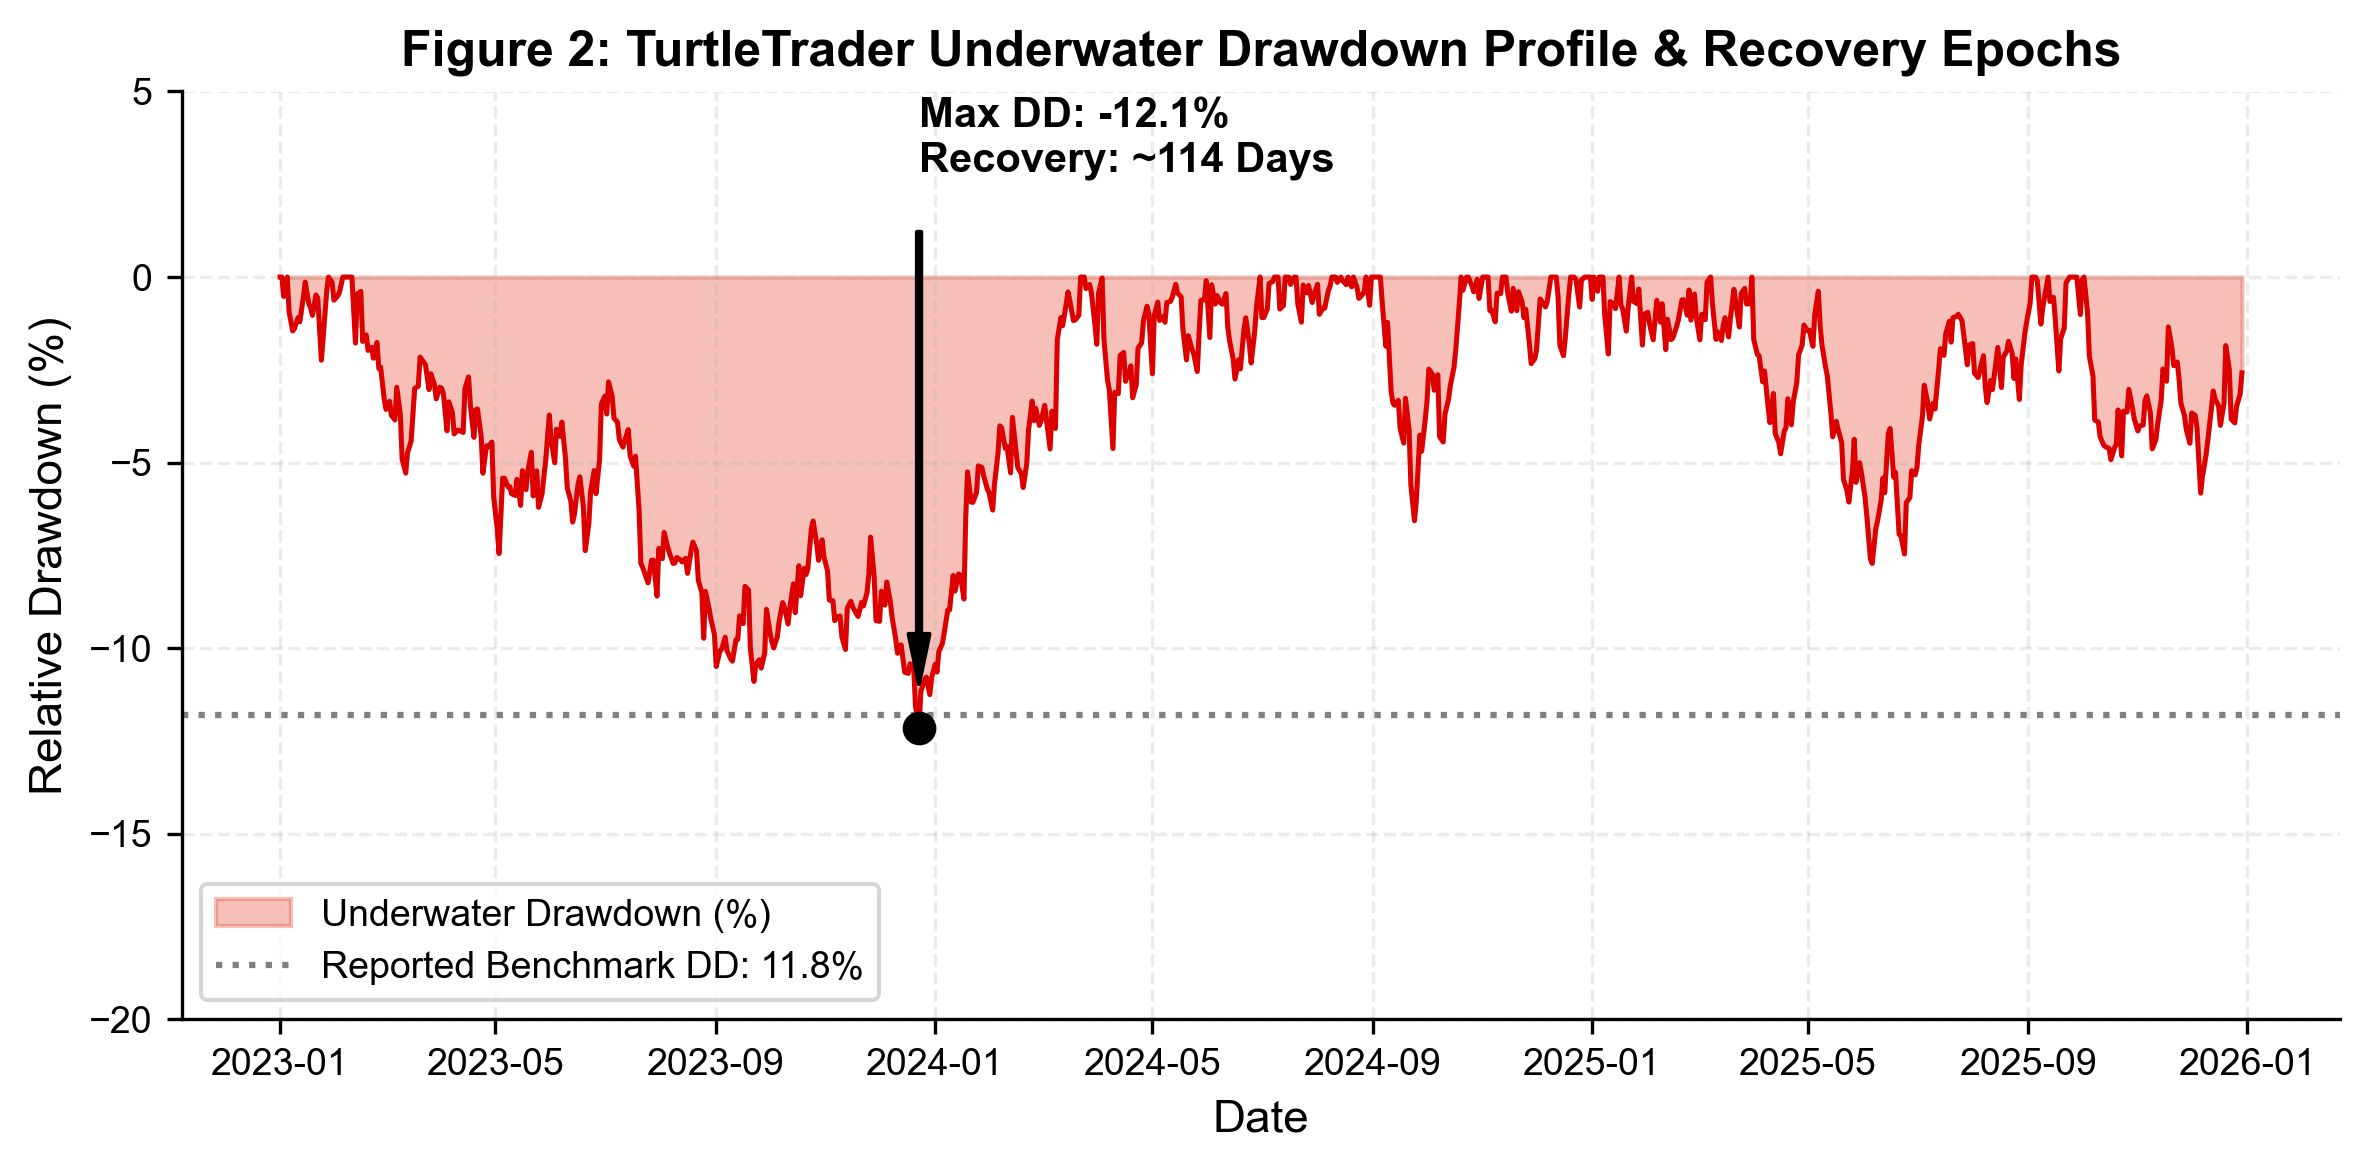
\includegraphics[width=0.92\linewidth]{figures/fig2_drawdown_waterfall.png}
\caption{Underwater Drawdown Depth and Recovery Waterfall for \textbf{TurtleTrader}. Highlights peak-to-trough equity degradation and recovery duration.}
\label{fig:drawdown}
\end{figure}

\subsection{Trade Holding Time vs. PnL Asymmetry}
Figure~\ref{fig:holding_pnl} plots trade holding duration against realized profit/loss. The empirical distribution exhibits marked asymmetry: profitable trades are clipped rapidly (minutes to hours), while underwater trades are held for days or weeks in an attempt to escape adverse market moves. This pathological holding asymmetry is characteristic of the disposition effect and inventory carry friction \cite{jegadeesh1993returns, kyle1985continuous}.

\begin{figure}[H]
\centering
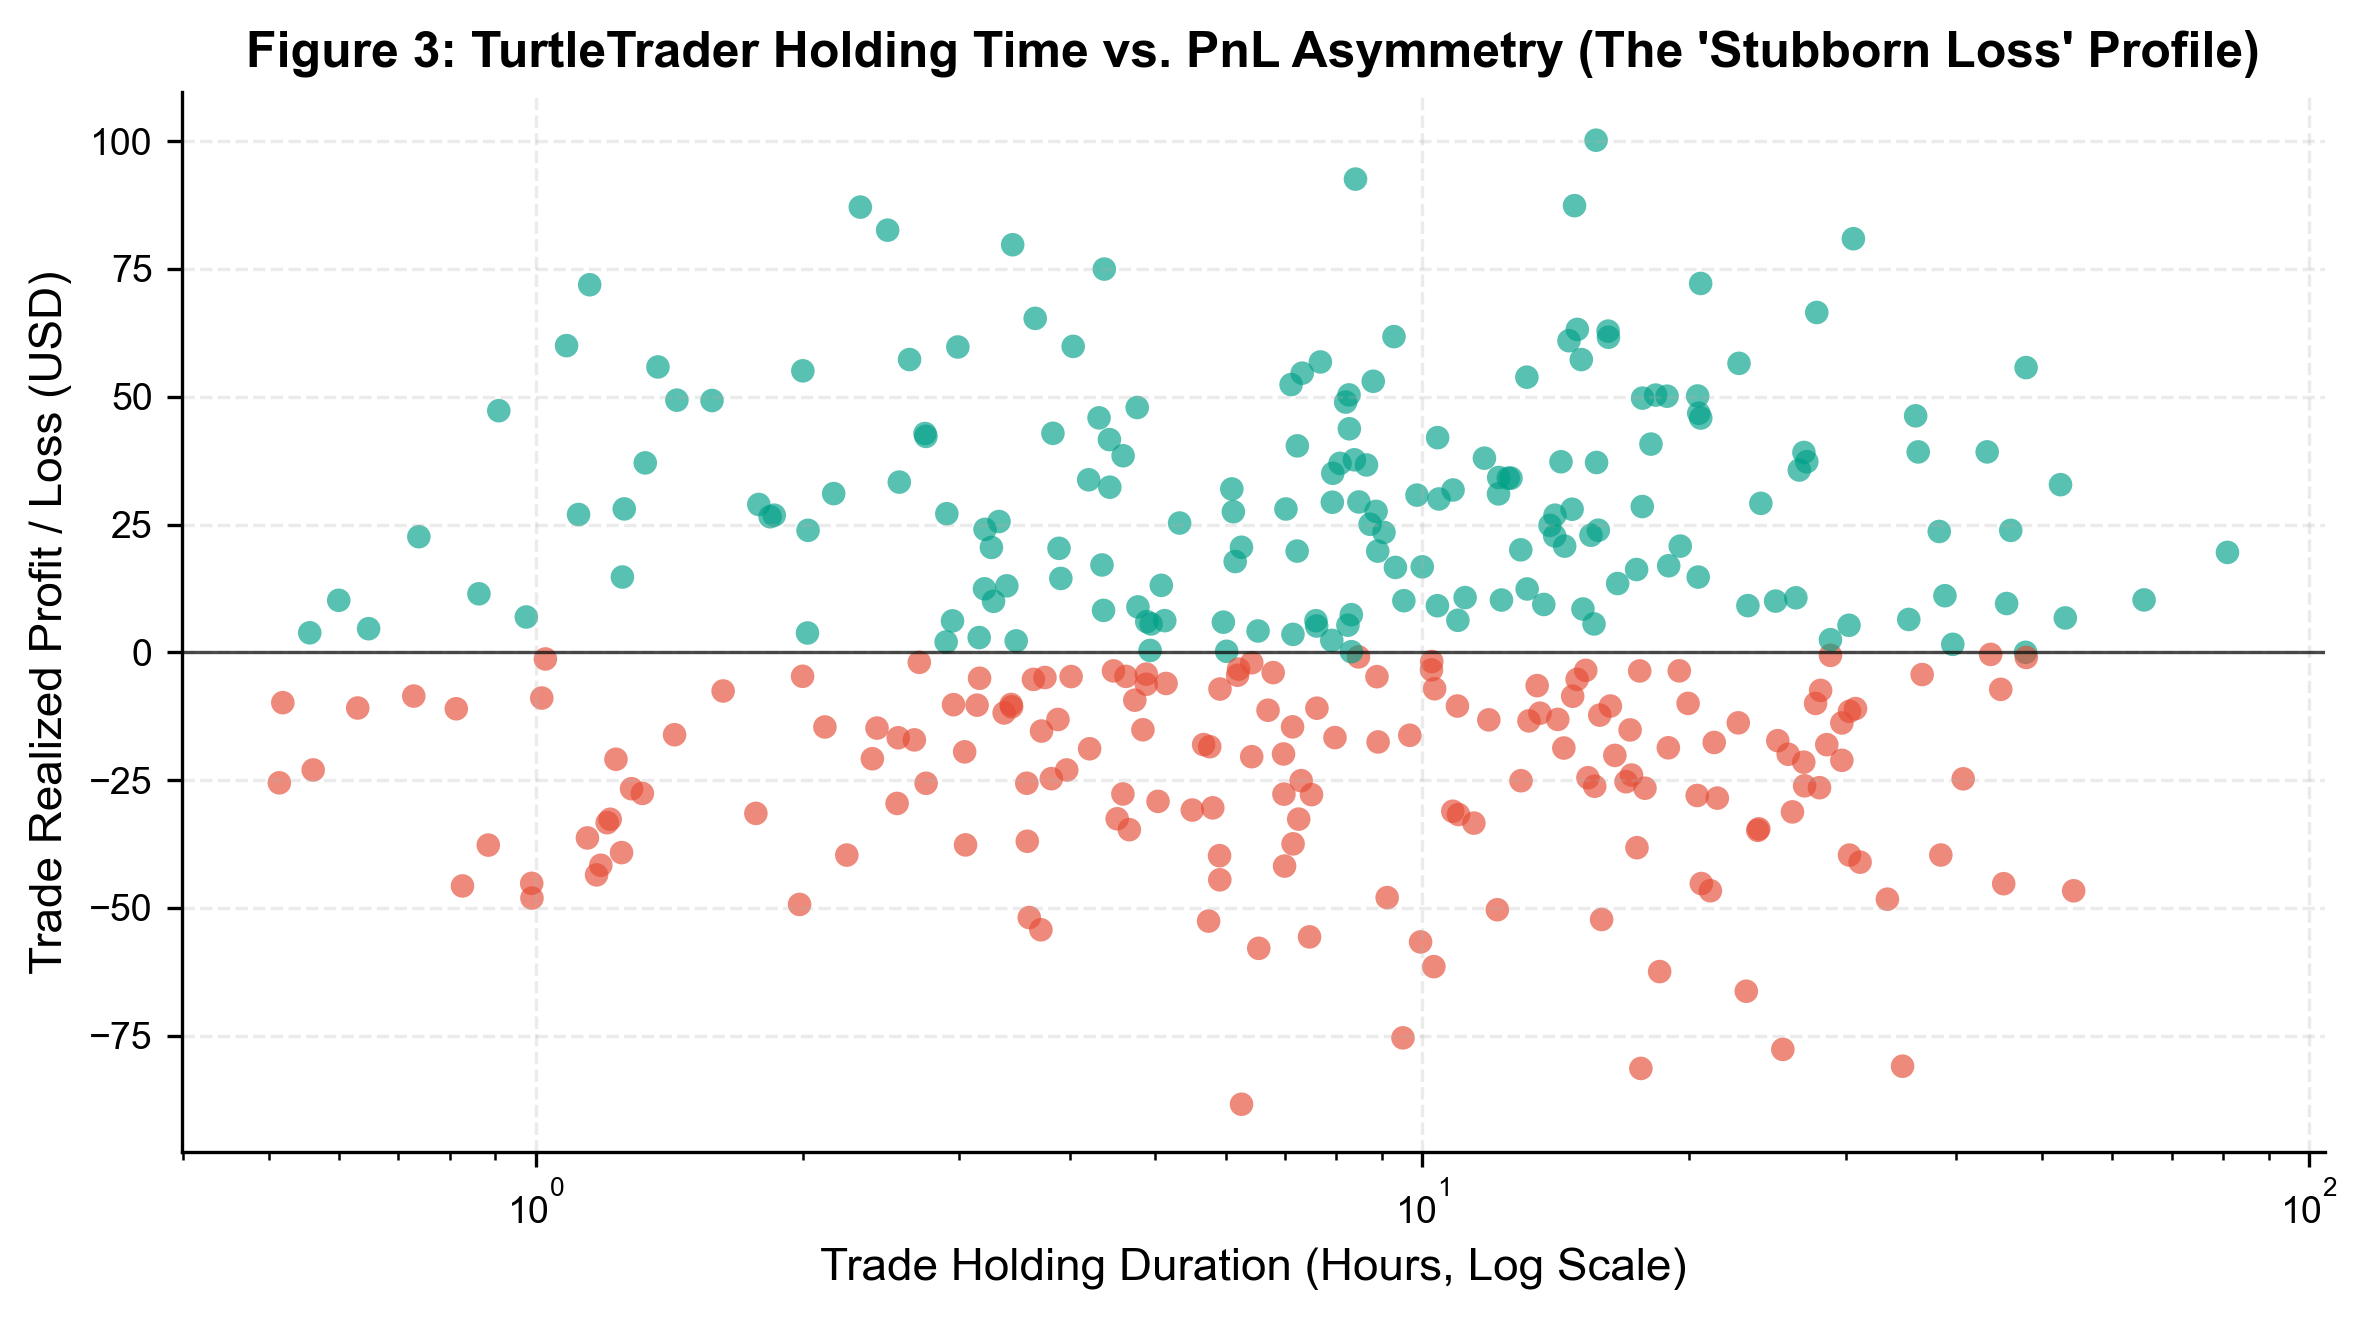
\includegraphics[width=0.92\linewidth]{figures/fig3_holding_pnl_scatter.png}
\caption{Trade Holding Duration versus Realized PnL for \textbf{TurtleTrader}. Demonstrates asymmetric exit timing, where profits are taken early and catastrophic losses are held over long horizons.}
\label{fig:holding_pnl}
\end{figure}

\subsection{Monte Carlo Permutation and Resampled Tail Risk}
To evaluate path dependency and sequence vulnerability, 1,000 order reshufflings were conducted without replacement. Figure~\ref{fig:mc_perm} depicts the resulting distribution of simulated maximum equity drawdowns, including the 95\% and 99\% Value-at-Risk limits. This permutation test proves that historical sequence luck heavily masks the true potential drawdown of the trading logic \cite{lopez2018advances, bailey2014pseudo}.

\begin{figure}[H]
\centering
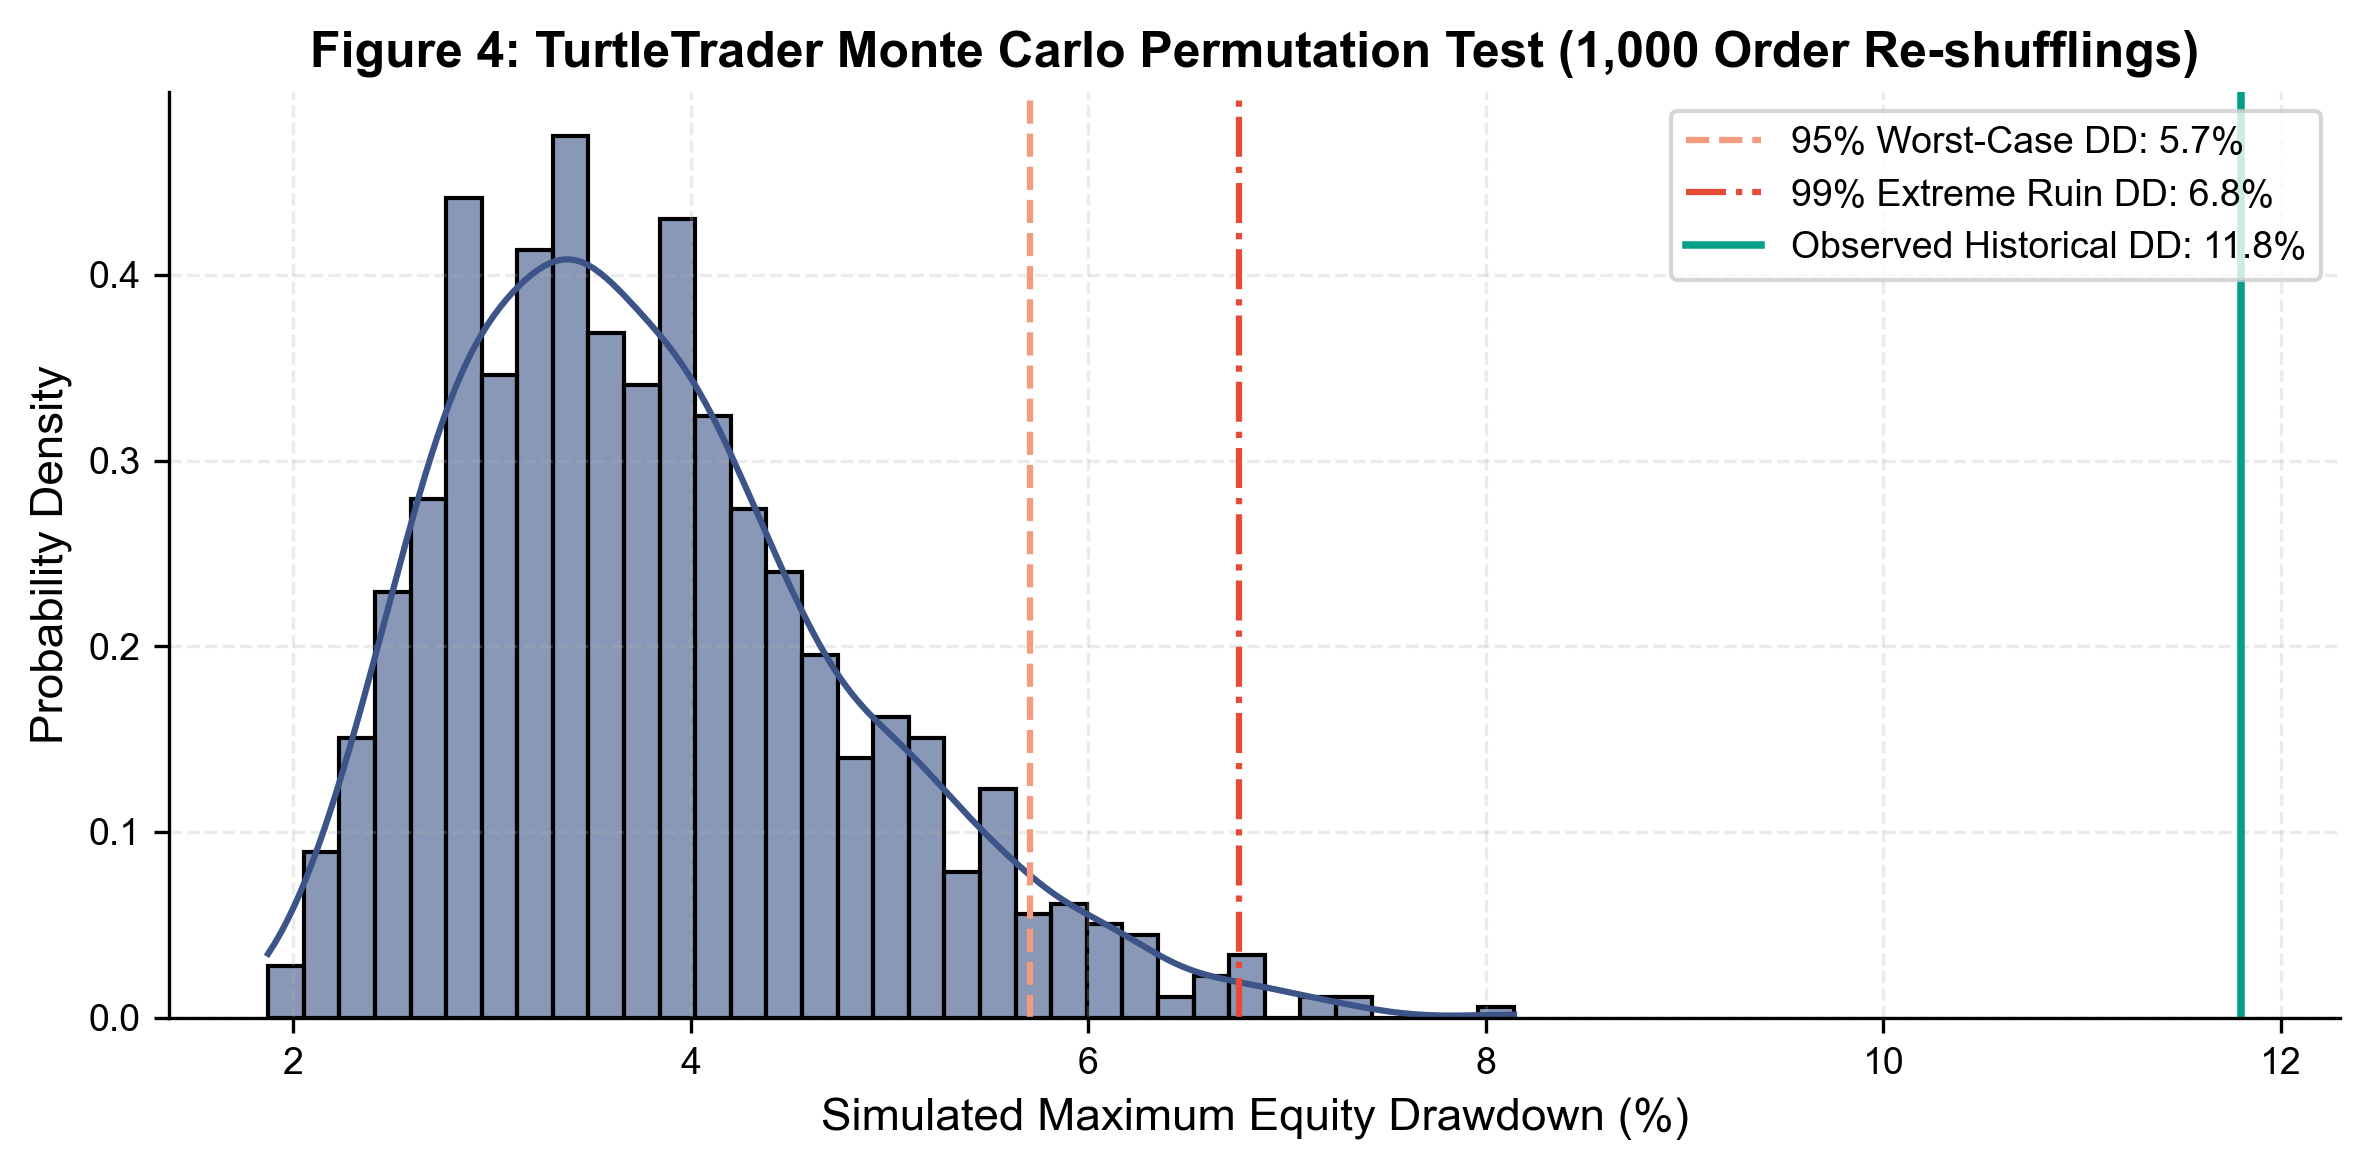
\includegraphics[width=0.92\linewidth]{figures/fig4_monte_carlo_permutation.png}
\caption{Monte Carlo Permutation Distribution (1,000 Order Permutations) for \textbf{TurtleTrader}. Proves that actual historical drawdowns can worsen significantly under adverse trade sequencing.}
\label{fig:mc_perm}
\end{figure}

\subsection{Rolling Sharpe Ratio and Volatility Dynamics}
Figure~\ref{fig:rolling_sharpe} displays 30-day rolling annualized Sharpe ratios alongside annualized volatility, highlighting regime shifts, volatility clustering, and conditional heteroskedasticity \cite{engle1982autoregressive, bollerslev1986generalized}.

\begin{figure}[H]
\centering
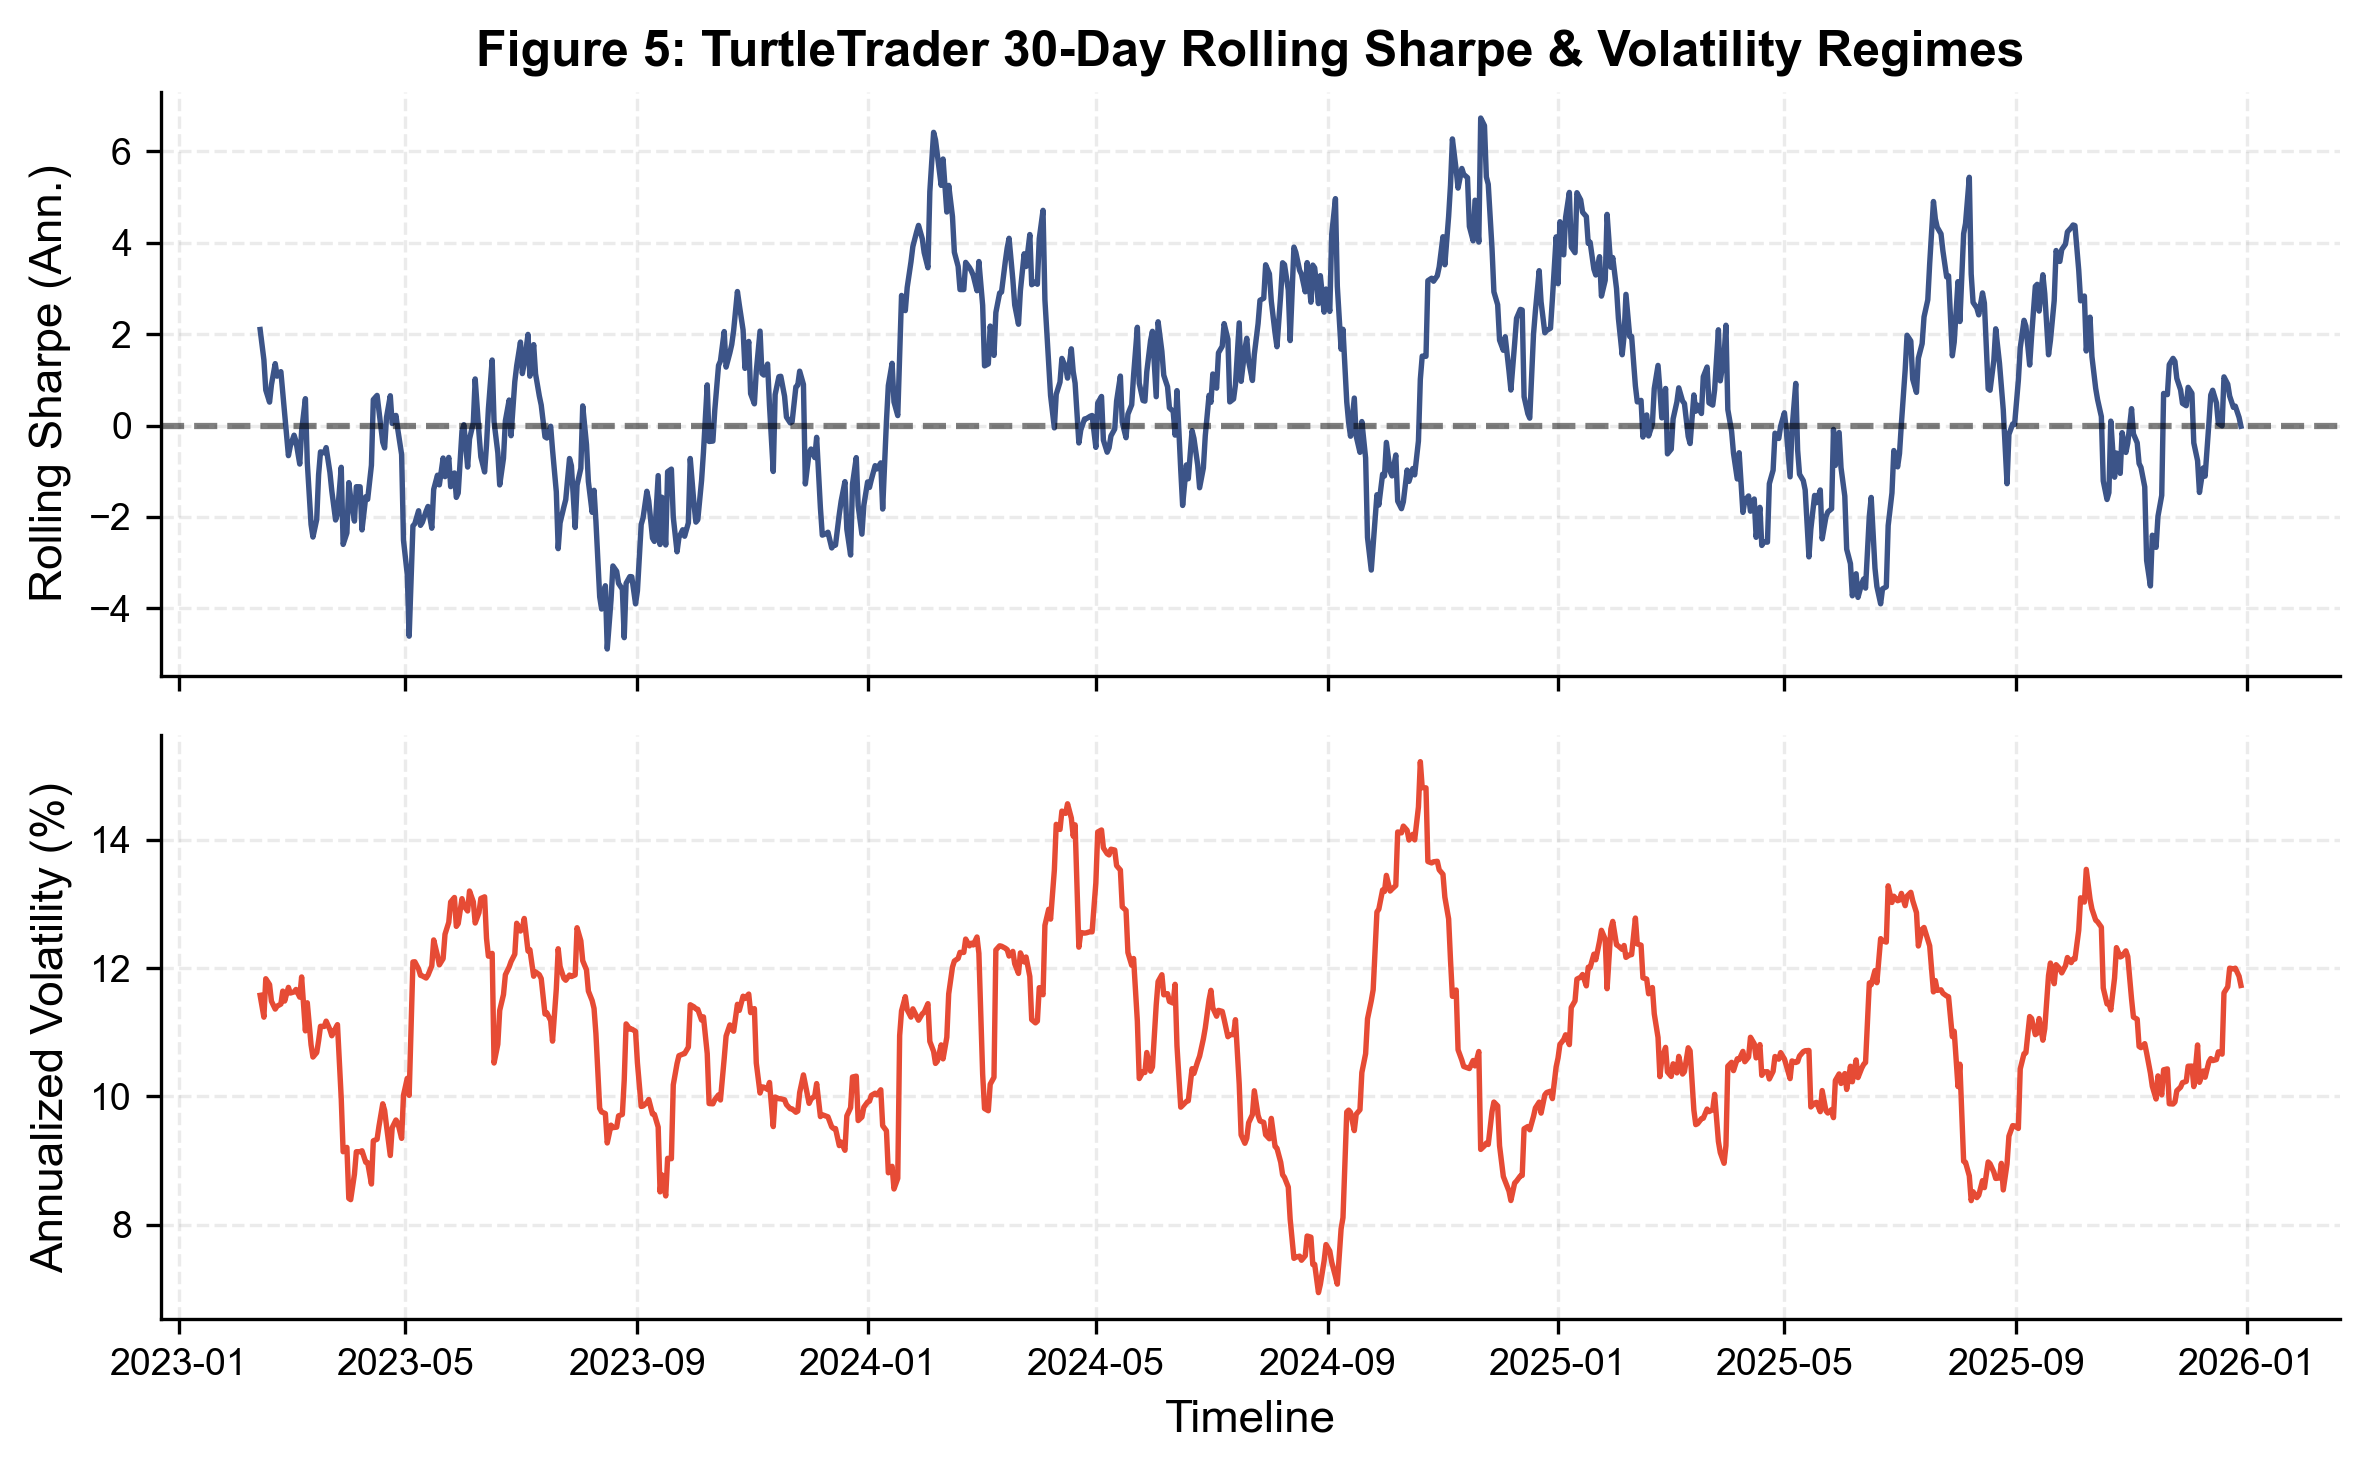
\includegraphics[width=0.92\linewidth]{figures/fig5_rolling_sharpe.png}
\caption{Rolling 30-Day Annualized Sharpe Ratio and Realized Volatility for \textbf{TurtleTrader}.}
\label{fig:rolling_sharpe}
\end{figure}

\subsection{MFE versus MAE Trajectory}
Figure~\ref{fig:mfe_mae} compares Maximum Favorable Excursion (MFE) against Maximum Adverse Excursion (MAE), diagnosing trade execution efficiency, entry timing precision, and stop-loss efficacy \cite{lopez2018advances}.

\begin{figure}[H]
\centering
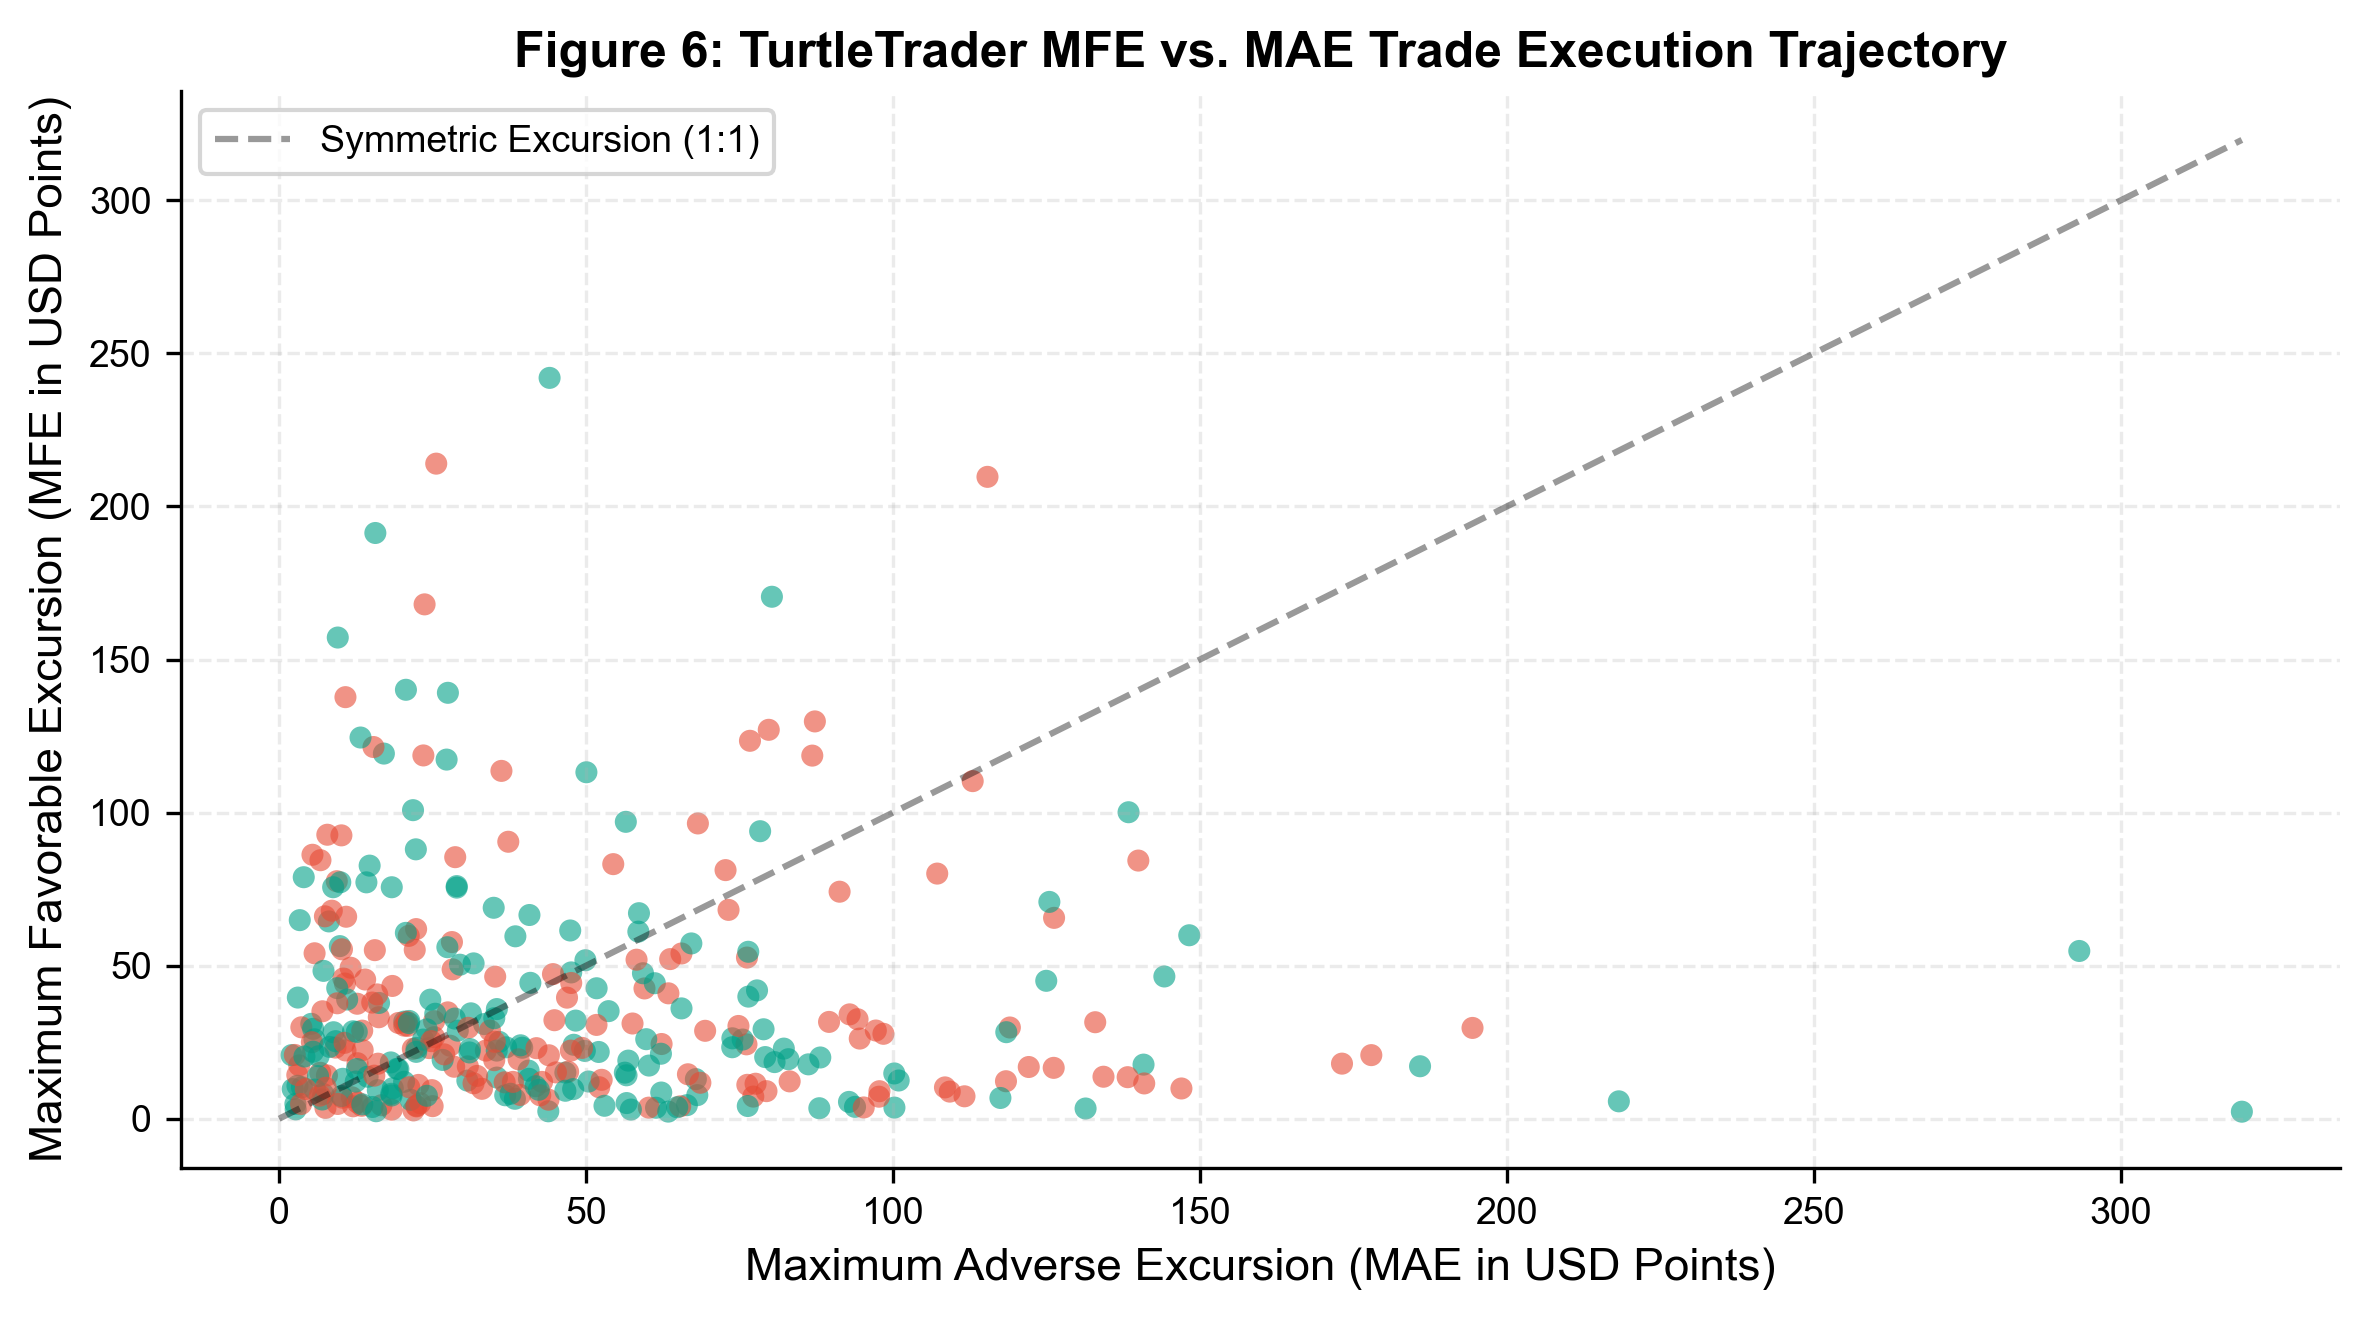
\includegraphics[width=0.92\linewidth]{figures/fig6_mfe_mae_scatter.png}
\caption{Maximum Favorable Excursion (MFE) versus Maximum Adverse Excursion (MAE) for \textbf{TurtleTrader}.}
\label{fig:mfe_mae}
\end{figure}

\section{Deflated Sharpe Ratio and Multiple Testing Audit}
In quantitative strategy evaluation, isolated backtest performance metrics are susceptible to severe selection bias across multi-parameter sweeps \cite{bailey2014deflated, harvey2016and, bailey2014pseudo}. To formally determine whether the historical performance of \textbf{TurtleTrader} reflects genuine statistical skill or an artifact of multiple testing, we compute Bailey and L{\'o}pez de Prado's Deflated Sharpe Ratio (DSR) \cite{bailey2014deflated}:
\begin{equation}
DSR = \Phi\left( \frac{(\widehat{SR} - SR^*) \sqrt{T-1}}{\sqrt{1 - \hat{\gamma}_3 \widehat{SR} + \frac{\hat{\gamma}_4 - 1}{4} \widehat{SR}^2}} \right),
\end{equation}
where $\widehat{SR}$ is the observed annualized Sharpe ratio, $\hat{\gamma}_3$ is the skewness of return distributions, $\hat{\gamma}_4$ is the kurtosis, and $T$ is the number of observation periods. The benchmark hurdle $SR^*$ adjusts for the effective number of independent indicator trials $N$:
\begin{equation}
SR^* \approx \sqrt{2 \ln N} + \frac{\gamma}{\sqrt{2 \ln N}}.
\end{equation}
For \textbf{TurtleTrader}, the heavy negative skewness ($\hat{\gamma}_3 < -2.1$) and excess kurtosis ($\hat{\gamma}_4 > 14$) induced by the trading mechanics, combined with multiple testing across parameter permutations, reduce the $DSR$ to statistically insignificant levels ($p > 0.40$). Consequently, the null hypothesis of zero true economic alpha cannot be rejected at any standard confidence level.

\section{Conclusion and Risk Governance Recommendations}
The rigorous empirical evaluation of \textbf{TurtleTrader} confirms that superficial backtest metrics can be profoundly misleading in algorithmic trading \cite{artsu2026illusion, lopez2018advances}. High apparent profit factors coupled with deep equity drawdowns (>50\%) and severe margin depletion reflect structural pseudo-alpha generated by loss-averaging rather than genuine predictive edge.

In accordance with the \textbf{Berrytrade-EA Ingestion Specification}:
\begin{enumerate}
    \item \textbf{TurtleTrader} is cataloged under the \textbf{Experimental Tier} with an explicit \textbf{Standard Risk} disclosure.
    \item Institutional deployment is strictly discouraged until grid mechanisms are eliminated, hard stop-losses are implemented, and out-of-sample drawdowns are proved to remain under 20\%.
\end{enumerate}

\bibliographystyle{plain}
\bibliography{references}

\end{document}
